% Options for packages loaded elsewhere
\PassOptionsToPackage{unicode}{hyperref}
\PassOptionsToPackage{hyphens}{url}
%
\documentclass[
  a4paper,
  openany]{article}
\usepackage{lmodern}
\usepackage{amssymb,amsmath}
\usepackage{ifxetex,ifluatex}
\ifnum 0\ifxetex 1\fi\ifluatex 1\fi=0 % if pdftex
  \usepackage[T1]{fontenc}
  \usepackage[utf8]{inputenc}
  \usepackage{textcomp} % provide euro and other symbols
\else % if luatex or xetex
  \usepackage{unicode-math}
  \defaultfontfeatures{Scale=MatchLowercase}
  \defaultfontfeatures[\rmfamily]{Ligatures=TeX,Scale=1}
\fi
% Use upquote if available, for straight quotes in verbatim environments
\IfFileExists{upquote.sty}{\usepackage{upquote}}{}
\IfFileExists{microtype.sty}{% use microtype if available
  \usepackage[]{microtype}
  \UseMicrotypeSet[protrusion]{basicmath} % disable protrusion for tt fonts
}{}
\makeatletter
\@ifundefined{KOMAClassName}{% if non-KOMA class
  \IfFileExists{parskip.sty}{%
    \usepackage{parskip}
  }{% else
    \setlength{\parindent}{0pt}
    \setlength{\parskip}{6pt plus 2pt minus 1pt}}
}{% if KOMA class
  \KOMAoptions{parskip=half}}
\makeatother
\usepackage{xcolor}
\IfFileExists{xurl.sty}{\usepackage{xurl}}{} % add URL line breaks if available
\IfFileExists{bookmark.sty}{\usepackage{bookmark}}{\usepackage{hyperref}}
\hypersetup{
  pdftitle={SPRAINED study},
  pdfauthor={Richard Pilbery, Tracey Young, Andrew Hodge},
  hidelinks,
  pdfcreator={LaTeX via pandoc}}
\urlstyle{same} % disable monospaced font for URLs
\usepackage[margin=2cm]{geometry}
\usepackage{longtable,booktabs}
% Correct order of tables after \paragraph or \subparagraph
\usepackage{etoolbox}
\makeatletter
\patchcmd\longtable{\par}{\if@noskipsec\mbox{}\fi\par}{}{}
\makeatother
% Allow footnotes in longtable head/foot
\IfFileExists{footnotehyper.sty}{\usepackage{footnotehyper}}{\usepackage{footnote}}
\makesavenoteenv{longtable}
\usepackage{graphicx,grffile}
\makeatletter
\def\maxwidth{\ifdim\Gin@nat@width>\linewidth\linewidth\else\Gin@nat@width\fi}
\def\maxheight{\ifdim\Gin@nat@height>\textheight\textheight\else\Gin@nat@height\fi}
\makeatother
% Scale images if necessary, so that they will not overflow the page
% margins by default, and it is still possible to overwrite the defaults
% using explicit options in \includegraphics[width, height, ...]{}
\setkeys{Gin}{width=\maxwidth,height=\maxheight,keepaspectratio}
% Set default figure placement to htbp
\makeatletter
\def\fps@figure{htbp}
\makeatother
\setlength{\emergencystretch}{3em} % prevent overfull lines
\providecommand{\tightlist}{%
  \setlength{\itemsep}{0pt}\setlength{\parskip}{0pt}}
\setcounter{secnumdepth}{5}
\usepackage{booktabs}
\usepackage{amsthm}
\usepackage{longtable}
\makeatletter
\def\thm@space@setup{%
  \thm@preskip=8pt plus 2pt minus 4pt
  \thm@postskip=\thm@preskip
}
\makeatother
\AtBeginDocument{\let\maketitle\relax} \usepackage{multirow}
\usepackage{booktabs}
\usepackage{longtable}
\usepackage{array}
\usepackage{multirow}
\usepackage{wrapfig}
\usepackage{float}
\usepackage{colortbl}
\usepackage{pdflscape}
\usepackage{tabu}
\usepackage{threeparttable}
\usepackage{threeparttablex}
\usepackage[normalem]{ulem}
\usepackage{makecell}
\usepackage{xcolor}

\title{SPRAINED study}
\author{Richard Pilbery, Tracey Young, Andrew Hodge}
\date{2020-07-17}

\begin{document}
\maketitle

{
\setcounter{tocdepth}{2}
\tableofcontents
}
\hypertarget{the-effect-of-a-specialist-paramedic-primary-care-rotation-on-appropriate-non-conveyance-decisions-a-controlled-interrupted-time-series-analysis}{%
\section*{The effect of a specialist paramedic primary care rotation on appropriate non-conveyance decisions: a controlled interrupted time series analysis}\label{the-effect-of-a-specialist-paramedic-primary-care-rotation-on-appropriate-non-conveyance-decisions-a-controlled-interrupted-time-series-analysis}}
\addcontentsline{toc}{section}{The effect of a specialist paramedic primary care rotation on appropriate non-conveyance decisions: a controlled interrupted time series analysis}

\hypertarget{author-information}{%
\subsection*{Author information}\label{author-information}}
\addcontentsline{toc}{subsection}{Author information}

\textbf{Richard Pilbery}\\
Research paramedic\\
Yorkshire Ambulance Service NHS Trust\\
Springhill, Brindley Way\\
Wakefield 41 Business Park\\
Wakefield\\
WF2 0XQ

ORCID: \url{https://orcid.org/0000-0002-5797-9788}

email: \href{mailto:r.pilbery@nhs.net}{\nolinkurl{r.pilbery@nhs.net}}\\
tel:

\textbf{Prof.~Tracey Young}\\
School of Health and Related Research, University of Sheffield

\textbf{Andrew Hodge}\\
Yorkshire Ambulance Service NHS Trust

\textbf{Keywords:} Paramedic rotation, Urgent care, Safe non-conveyance

\hypertarget{abstract}{%
\subsection*{Abstract}\label{abstract}}
\addcontentsline{toc}{subsection}{Abstract}

\hypertarget{introduction}{%
\subsubsection*{Introduction}\label{introduction}}
\addcontentsline{toc}{subsubsection}{Introduction}

Ambulance conveyance rates in the UK NHS are almost 70\%, despite an increase in non-emergency cases. This is increasing the demands on crowded emergency departments (ED) and contributes to increased ambulance turnaround times. Yorkshire Ambulance Service introduced a specialist paramedic (SP) role to try and address this, but non-conveyance rates in this group have not been much greater than regular paramedics.

\hypertarget{methods}{%
\subsubsection*{Methods}\label{methods}}
\addcontentsline{toc}{subsubsection}{Methods}

We conducted a controlled interrupted time series analysis to study appropriate non-conveyance rates before and after the GP rotation. A costing analysis examined the average cost per appropriate non-conveyance achieved for patients receiving care from intervention group SPs compared to a matched control group.

\hypertarget{results}{%
\subsubsection*{Results}\label{results}}
\addcontentsline{toc}{subsubsection}{Results}

Between June 2017 and December 2019 there were 7349 incidents attended by intervention group SPs and eligible for inclusion. Following removal of cases with missing data, 5537/7349 (75.3\%) cases remained. Post-placement, the intervention group demonstrated an increase in appropriate non-conveyance rate by 35.0\% (95\%CI 23.8--46.2\%, p=\textless0.001) and a reduction in the trend of appropriate non-conveyance relative to the control group of -1.2\% (95\%CI -2.8--0.5\%, p=0.156).

Post-rotation, intervention group SPs cost a mean of £323.71 per incident (95\% CI £318.77--£328.88), compared to £347.79 per incident (95\% CI £343.48--£351.81) for the control group. Cost per appropriate non-conveyance for intervention SPs was a mean of £509.42 (95\%CI £485.04--£534.97) versus £1124.41 (95\%CI £1042.89--£1216.95) for the control group.

\hypertarget{conclusion}{%
\subsubsection*{Conclusion}\label{conclusion}}
\addcontentsline{toc}{subsubsection}{Conclusion}

In this single NHS ambulance service study, we found a clinically and statistical significant increase in appropriate non-conveyance rates by SPs who had completed a 10-week GP rotation. This improvement persisted for the 12-month period following the rotation and was cheaper compared to usual care.

\hypertarget{introduction-1}{%
\section*{Introduction}\label{introduction-1}}
\addcontentsline{toc}{section}{Introduction}

The National Health Service (NHS) in the United Kingdom is facing a 5\% year-on-year increase in demand for urgent and emergency care services {[}\protect\hyperlink{ref-national_audit_office_nhs_2017}{1}{]}. In 2018/19, ambulance services in England provided a face-to-face assessment to nearly 7.9 million incidents, of which 7.6 million were conveyed to hospital {[}\protect\hyperlink{ref-nhs_england_ambulance_2019}{2}{]}. This conveyance rate of around 69\% is occurring despite an increase in non-emergency cases and is placing increasing demands on already crowded emergency departments (EDs), leading to decreased availability of ambulances as turnaround times at hospitals increase {[}\protect\hyperlink{ref-willett_addressing_2017}{3}{]}. ED overcrowding is a significant issue for patients, resulting in poorer quality of care, increased healthcare costs and potentially, increased mortality {[}\protect\hyperlink{ref-sun_effect_2013}{4}--\protect\hyperlink{ref-richardson_increase_2006}{7}{]}.

Yorkshire Ambulance Service have been early adopters of initiatives to address inappropriate conveyance, and have had advanced paramedics working in the role of Emergency Care Practitioners (ECP), since 2004 {[}\protect\hyperlink{ref-mason_developing_2003}{8}{]}. Even without selective dispatching, ECPs consistently have non-conveyance rates double that of other paramedics in the Trust. More recently, the specialist paramedic (SP) role has been introduced, with education comprising of a 1 year university program. However, SP non-conveyance rates have been only marginally better compared to other paramedics within the Trust.

In 2018, Health Education England funded a pilot scheme to rotate paramedics into a range of healthcare settings, with the aim of improving patient care and relieving pressures on primary care, ambulance services and other parts of the NHS in a sustainable way {[}\protect\hyperlink{ref-turner_evaluation_2018}{9}{]}. However, to date no cost-effectiveness analysis of the scheme has been published.

This pilot presented an opportunity to develop SPs and further improve their decision-making, with potential to deliver the patient and cost-benefits of the role as originally anticipated.

This study aimed to evaluate whether specialist paramedics who have rotated into primary care, are appropriately increasing the level and trend of non-conveyance decisions compared to a matched control population of YAS paramedics and are cost-effective.

\hypertarget{objectives}{%
\subsection*{Objectives}\label{objectives}}
\addcontentsline{toc}{subsection}{Objectives}

The primary objective was to determine the change and trend in proportion of appropriate non-conveyance decisions by specialist paramedics who have completed a 10-week rotation in a GP surgery. The secondary objective was to compare the cost-effectiveness between specialist paramedics who have completed a 10-week rotation in a GP surgery and a matched control group of YAS paramedics.

\hypertarget{methods-1}{%
\section*{Methods}\label{methods-1}}
\addcontentsline{toc}{section}{Methods}

This study was a natural experiment using routinely collected observational data. We utilised a controlled interrupted time series analysis method to detect any change in the level and trend of paramedic appropriate non-conveyance decisions. The cost-effectiveness analysis examined the cost per appropriate non-conveyance achieved for patients receiving care from specialist paramedics who have completed a 10 week rotation in a GP surgery compared with those receiving care from paramedics who did not take part in the primary care rotational pilot.

\hypertarget{setting}{%
\subsection*{Setting}\label{setting}}
\addcontentsline{toc}{subsection}{Setting}

Yorkshire Ambulance Service NHS Trust (YAS) provides 24-hour emergency and health care services for the county of Yorkshire in northern England. The county has a population of approximately five million, spread over almost 6000 square miles of varied terrain, included isolated moors and dales, coastline and heavily populated urban areas. In 2018/19 YAS received more than 998,500 emergency calls and responded to 798,968 incidents through either a vehicle arriving on scene or by telephone advice.

\hypertarget{specialist-paramedic-rotation}{%
\subsubsection*{Specialist paramedic rotation}\label{specialist-paramedic-rotation}}
\addcontentsline{toc}{subsubsection}{Specialist paramedic rotation}

YAS employs approximately 118 specialist paramedics (SPs) and emergency care practitioners (ECPs). 30 clinicians took part in the rotational paramedic pilot across different sites, with the largest scheme comprising 5 ECPs and 10 SPs working with Leeds Primary Care. The ECPs and SPs rotated between providing a home visiting service for 15 GP surgeries, front line operations (999) and the emergency operations centre (EOC).

\hypertarget{data-sources}{%
\subsection*{Data sources}\label{data-sources}}
\addcontentsline{toc}{subsection}{Data sources}

We used routinely collected computer aided dispatch (CAD) and patient record data to identify all cases attended by one of the 10 SPs who had completed a GP placement in the Leeds area. For operational reasons, these placements were staggered, with the first paramedics entering the rotation in June 2018 and the final paramedics completed their placements at the end of December 2018. In order to obtain sufficient data pre- and post-pilot, all cases attended by these paramedics in the 12 month period prior to the rotation commencing, and 12 months after the placement had completed, were obtained. To count as an `attendance', the SP's name had to appear on the patient record.

To take account of case-mix and paramedic experience in the pre- and post-rotational phase, a matched comparison (control) group consisting of cases in Yorkshire covering the period from the 1st June, 2017 to 31st December, 2019 was obtained. This cohort of patients received a face-to-face assessment by paramedics who did not take part in the GP rotation.

Since YAS does not keep a record of paramedic registration beyond the current 2-year registration cycle, it was not possible to determine how long staff had been registered as a paramedic. Instead, we identified when staff were first entered into the Health and Professions Council (HCPC) paramedic register.

\hypertarget{study-variables}{%
\subsection*{Study variables}\label{study-variables}}
\addcontentsline{toc}{subsection}{Study variables}

We hypothesised that appropriate non-conveyance was likely to increase following the 10-week placement, but needed to ensure that we took account of factors previously identified as being important for pre-hospital clinicians making non-conveyance decisions {[}\protect\hyperlink{ref-ocathain_understanding_2018}{10}{]}. To achieve this, we aimed to match the control and intervention groups on the following variables:

\begin{itemize}
\tightlist
\item
  Patient:

  \begin{itemize}
  \tightlist
  \item
    Age (5 year increments)
  \item
    Sex
  \item
    Working impression (as determined by paramedic on scene)
  \item
    Time of call (in-hours/out-of-hours)
  \item
    Call category
  \item
    Call month and year
  \item
    Lowest National Early Warning Score (NEWS) threshold
  \end{itemize}
\item
  Location (lower super output area, LSOA):

  \begin{itemize}
  \tightlist
  \item
    Urban/rural
  \item
    Index of multiple deprivation decile
  \item
    Proportion of population within LSOA with a long-term physical or mental illness (0--4\%, 4--8\%, 8--12\%)
  \end{itemize}
\item
  Paramedics

  \begin{itemize}
  \tightlist
  \item
    Years registered as a paramedic (\textless1 year, 1--5 years, \textgreater5 years)
  \item
    Role designation at time of incident.
  \end{itemize}
\end{itemize}

Since the ambulance service does not routinely capture outcome data for patients, we pragmatically defined appropriate non-conveyance as any patient episode where the patient was not transferred to hospital and no further calls were made to the ambulance service in the following 72 hours.

\hypertarget{matching}{%
\subsection*{Matching}\label{matching}}
\addcontentsline{toc}{subsection}{Matching}

Matching was performed utilising a genetic algorithm and computed using the `Matching' R statistics package {[}\protect\hyperlink{ref-sekhon_multivariate_2011}{11}{]}. Genetic algorithms are a subgroup of evolutionary computing which as the name suggests, imitate biological processes of reproduction and natural selection to solve according to `fitness' {[}\protect\hyperlink{ref-mitchell_introduction_1996}{12}{]}. The `Matching' package uses this algorithm to find the optimal balance between groups by examining the cumulative probability distribution functions of a variety of standardised statistics such as t-tests and Kolmogorov-Smirnov tests.

Cases where the patient record could not be located, or where data was missing were excluded. With the exception of ECPs (who were removed since their non-conveyance rates are consistently higher than other clinicians), it was not possible to accurately determine what role designation paramedics in the control group had. As a result, this was removed as a matching variable.

\hypertarget{statistical-methods}{%
\subsection*{Statistical methods}\label{statistical-methods}}
\addcontentsline{toc}{subsection}{Statistical methods}

\hypertarget{sample-size-calculation}{%
\subsubsection*{Sample size calculation}\label{sample-size-calculation}}
\addcontentsline{toc}{subsubsection}{Sample size calculation}

The sample size was constrained by the fact that this was an observational study with only 12 months pre- and post- rotation available. Based on a previous audit of 999 call data, we anticipated that there would be approximately 700 patient episodes per month. Given that the time series analysis included data from 24 months in total, this resulted in an estimated 33,600 patients.

\hypertarget{summary-of-baseline-data}{%
\subsubsection*{Summary of baseline data}\label{summary-of-baseline-data}}
\addcontentsline{toc}{subsubsection}{Summary of baseline data}

Descriptive statistics were used to summarise the data pre- and post-rotation and between rotational paramedics and non-rotational paramedics, to illustrate the success of matching. Median and interquartile ranges were reported for continuous variables, and counts and proportions reported for categorical data.

\hypertarget{primary-outcome-analysis}{%
\subsubsection*{Primary outcome analysis}\label{primary-outcome-analysis}}
\addcontentsline{toc}{subsubsection}{Primary outcome analysis}

We conducted a retrospective analysis of appropriate non-conveyance before and after the GP rotation, using segmented regression as part of a controlled interrupted time series (CITS) design {[}\protect\hyperlink{ref-penfold_use_2013}{13}{]}. Since the SP placements were staggered, the actual month and year was not utilised. Instead, the number of months before and after the placement were used, so that month 1 was the month that occurred 12 months prior to the GP placement for all SPs and month 24, the month that occurred 12 months after the placement. It was anticipated that this would remove or reduce any autocorrelation. However, we checked for autoregression and moving averages by performing the Durbin-Watson test and by plotting autocorrelation function and partial autocorrelation function plots. Coefficients from the model were used to predict the absolute and relative changes in appropriate non-conveyance immediately after the 10-week placement and at 12-months.

\hypertarget{secondary-outcome-analysis}{%
\subsubsection*{Secondary outcome analysis}\label{secondary-outcome-analysis}}
\addcontentsline{toc}{subsubsection}{Secondary outcome analysis}

Salary costs were calculated for the 10 week GP placement and divided by the number of incidents attended by SPs to calculate a per-incident cost. SPs were assumed to be salaried at NHS Agenda for Change mid-band 6, which was £31,121 for 2018/19. Education costs were not included since all SPs had already undertaken the education component prior to the rotation commencing. The resource use related to the dispatch of the ambulance, cost of conveyance and admission to the ED was calculated using reference costs published by the NHS Improvement reference costs {[}\protect\hyperlink{ref-nhs_improvement_reference_2018}{14}{]} (Table \ref{tab:callcosts}. For example, a non-conveyance would comprise the cost of answering a 999 call and an ambulance: see and treat. In the event that a recall was made within 72 hours, the total cost for the non-conveyance would be the 999 call, ambulance: see and treat plus the cost of the second call i.e.~999 call and ambulance (see and treat or see, treat and convey plus ED attendance).

\begin{longtable}[t]{ll}
\caption{\label{tab:callcosts}Unit costs to the NHS for ambulance 999 calls}\\
\toprule
item & cost\\
\midrule
\endfirsthead
\caption[]{\label{tab:callcosts}Unit costs to the NHS for ambulance 999 calls \textit{(continued)}}\\
\toprule
item & cost\\
\midrule
\endhead
\
\endfoot
\bottomrule
\endlastfoot
\rowcolor{gray!6}  999 call & £7.33\\
Ambulance: see and treat & £209.38\\
\rowcolor{gray!6}  Ambulance: see, treat and convey & £257.34\\
ED attendance & £135.00\\*
\end{longtable}

Bootstrapping was used to estimate uncertainty (95\% confidence intervals) around cost estimates. Costs of those patients seen by paramedics undertaking the 10-week training rotation was compared with matched controls and the results presented as the cost per appropriate conveyance.

\hypertarget{results-1}{%
\section*{Results}\label{results-1}}
\addcontentsline{toc}{section}{Results}

As part of the Health Education England rotational paramedic pilot, 10 specialist paramedics undertook a 10 week placement in a primary care setting in the Leeds area. Five paramedics commenced their placement in June 2018, with a further three starting in August 2018 and the final two starting their placement in October 2018.

Between 1st June 2017 and 31st December, 2019 there were 8849 incidents attended by one of the rotational paramedics. Once data was adjusted to remove any cases occurring in the 10 week rotation period, and outside of the 12 months prior to the start of the rotation and 12 months after the end of the rotation, 7349 cases remained. A further 6 had no gender recorded, 15 had no age recorded and 8 had no post code, leaving 7326/7349 (99.7\%) cases. A further 4 cases were excluded due to a missing index of multiple deprivation decile (3 cases), rural urban classification (3 cases) and/or prevalence of missing long-term condition data (4 cases), leaving 7322/7349 (99.6\%) cases. Finally, no working impression was included in 1785 cases, resulting in a final dataset of 5537/7349 (75.3\%) cases for inclusion in the final analysis. Due to the high number of missing working impressions, a sensitivity analysis was performed excluding the working impression as a variable (Appendix 1).

\hypertarget{matched-dataset-for-analysis}{%
\subsection*{Matched dataset for analysis}\label{matched-dataset-for-analysis}}
\addcontentsline{toc}{subsection}{Matched dataset for analysis}

The matching algorithm utilised 5198/5537 (93.9\%) cases. Overall, the control group was closely matched to the rotational paramedic (intervention group) incidents (defined as less than 10\% in standardised mean difference). Only the NEWS risk category and prevalence of long-term conditions were outside this limit.

\hypertarget{pre--and-post-rotation-exploratory-data-analysis}{%
\subsection*{Pre- and Post-rotation exploratory data analysis}\label{pre--and-post-rotation-exploratory-data-analysis}}
\addcontentsline{toc}{subsection}{Pre- and Post-rotation exploratory data analysis}

In addition to the substantial reduction in number of cases attended post-rotation, there were also other differences in pre- and post-rotation cases, which could have contributed to the change in rate of non-conveyance, validating the decision to include a matched control (Table \ref{tab:table1}).

\begin{longtable}[t]{lllll}
\caption{\label{tab:table1}Comparison of matched control and rotational paramedic groups, stratified by pre and post-placement phases}\\
\toprule
\multicolumn{1}{c}{ } & \multicolumn{2}{c}{Pre-placement} & \multicolumn{2}{c}{Post-placement} \\
\cmidrule(l{3pt}r{3pt}){2-3} \cmidrule(l{3pt}r{3pt}){4-5}
Measure & Control & Intervention & Control & Intervention\\
\midrule
\endfirsthead
\caption[]{\label{tab:table1}Comparison of matched control and rotational paramedic groups, stratified by pre and post-placement phases \textit{(continued)}}\\
\toprule
Measure & Control & Intervention & Control & Intervention\\
\midrule
\endhead
\
\endfoot
\bottomrule
\endlastfoot
\rowcolor{gray!6}  n & 3297 & 3297 & 1901 & 1901\\
Appropriately not conveyed n (\%) & 582 (17.7) & 924 (28.0) & 588 (30.9) & 1208 (63.5)\\
\rowcolor{gray!6}  Not conveyed n (\%) & 635 (19.3) & 1012 (30.7) & 653 (34.4) & 1342 (70.6)\\
\addlinespace[0.3em]
\multicolumn{5}{l}{\textbf{Yearly quarter n (\%)}}\\
\hspace{1em}1 & 902 (27.4) & 902 (27.4) & 285 (15.0) & 286 (15.0)\\
\rowcolor{gray!6}  \hspace{1em}2 & 713 (21.6) & 713 (21.6) & 451 (23.7) & 450 (23.7)\\
\hspace{1em}3 & 751 (22.8) & 751 (22.8) & 615 (32.4) & 614 (32.3)\\
\rowcolor{gray!6}  \hspace{1em}4 & 931 (28.2) & 931 (28.2) & 550 (28.9) & 551 (29.0)\\
Out-of-hours n (\%) & 2014 (61.1) & 1966 (59.6) & 1109 (58.3) & 1107 (58.2)\\
\rowcolor{gray!6}  \addlinespace[0.3em]
\multicolumn{5}{l}{\textbf{Call category}}\\
\hspace{1em}cat1 & 454 (13.8) & 640 (19.4) & 158 ( 8.3) & 168 ( 8.8)\\
\hspace{1em}cat2 & 2080 (63.1) & 1834 (55.6) & 866 (45.6) & 837 (44.0)\\
\rowcolor{gray!6}  \hspace{1em}cat3 & 676 (20.5) & 691 (21.0) & 629 (33.1) & 595 (31.3)\\
\hspace{1em}cat4 & 81 ( 2.5) & 97 ( 2.9) & 182 ( 9.6) & 222 (11.7)\\
\rowcolor{gray!6}  \hspace{1em}cat5 & 6 ( 0.2) & 35 ( 1.1) & 66 ( 3.5) & 79 ( 4.2)\\
Urban location n (\%) & 2985 (90.5) & 3007 (91.2) & 1792 (94.3) & 1787 (94.0)\\
\rowcolor{gray!6}  \addlinespace[0.3em]
\multicolumn{5}{l}{\textbf{IMD decile n (\%)}}\\
\hspace{1em}1 & 828 (25.1) & 967 (29.3) & 567 (29.8) & 624 (32.8)\\
\hspace{1em}2 & 464 (14.1) & 429 (13.0) & 277 (14.6) & 231 (12.2)\\
\rowcolor{gray!6}  \hspace{1em}3 & 363 (11.0) & 398 (12.1) & 219 (11.5) & 239 (12.6)\\
\hspace{1em}4 & 323 ( 9.8) & 204 ( 6.2) & 138 ( 7.3) & 87 ( 4.6)\\
\rowcolor{gray!6}  \hspace{1em}5 & 265 ( 8.0) & 276 ( 8.4) & 173 ( 9.1) & 158 ( 8.3)\\
\hspace{1em}6 & 265 ( 8.0) & 199 ( 6.0) & 136 ( 7.2) & 133 ( 7.0)\\
\rowcolor{gray!6}  \hspace{1em}7 & 278 ( 8.4) & 302 ( 9.2) & 152 ( 8.0) & 172 ( 9.0)\\
\hspace{1em}8 & 223 ( 6.8) & 182 ( 5.5) & 117 ( 6.2) & 102 ( 5.4)\\
\rowcolor{gray!6}  \hspace{1em}9 & 138 ( 4.2) & 181 ( 5.5) & 73 ( 3.8) & 92 ( 4.8)\\
\hspace{1em}10 & 150 ( 4.5) & 159 ( 4.8) & 49 ( 2.6) & 63 ( 3.3)\\
\rowcolor{gray!6}  \addlinespace[0.3em]
\multicolumn{5}{l}{\textbf{Prevalence of Long-term conditions n (\%)}}\\
\hspace{1em}[0,4] & 16 ( 0.5) & 43 ( 1.3) & 16 ( 0.8) & 27 ( 1.4)\\
\hspace{1em}(4,8] & 124 ( 3.8) & 423 (12.8) & 277 (14.6) & 275 (14.5)\\
\rowcolor{gray!6}  \hspace{1em}(8,12] & 3016 (91.5) & 2666 (80.9) & 1559 (82.0) & 1548 (81.4)\\
\hspace{1em}(12,16] & 141 ( 4.3) & 165 ( 5.0) & 49 ( 2.6) & 51 ( 2.7)\\
\rowcolor{gray!6}  \addlinespace[0.3em]
\multicolumn{5}{l}{\textbf{Patient age in years n (\%)}}\\
\hspace{1em}[0,5] & 24 ( 0.7) & 188 ( 5.7) & 49 ( 2.6) & 53 ( 2.8)\\
\hspace{1em}(5,10] & 17 ( 0.5) & 54 ( 1.6) & 26 ( 1.4) & 24 ( 1.3)\\
\rowcolor{gray!6}  \hspace{1em}(10,15] & 54 ( 1.6) & 60 ( 1.8) & 14 ( 0.7) & 35 ( 1.8)\\
\hspace{1em}(15,20] & 151 ( 4.6) & 153 ( 4.6) & 65 ( 3.4) & 70 ( 3.7)\\
\rowcolor{gray!6}  \hspace{1em}(20,25] & 192 ( 5.8) & 182 ( 5.5) & 114 ( 6.0) & 101 ( 5.3)\\
\hspace{1em}(25,30] & 186 ( 5.6) & 173 ( 5.2) & 105 ( 5.5) & 102 ( 5.4)\\
\rowcolor{gray!6}  \hspace{1em}(30,35] & 166 ( 5.0) & 168 ( 5.1) & 93 ( 4.9) & 103 ( 5.4)\\
\hspace{1em}(35,40] & 156 ( 4.7) & 168 ( 5.1) & 66 ( 3.5) & 72 ( 3.8)\\
\rowcolor{gray!6}  \hspace{1em}(40,45] & 161 ( 4.9) & 148 ( 4.5) & 66 ( 3.5) & 76 ( 4.0)\\
\hspace{1em}(45,50] & 206 ( 6.2) & 200 ( 6.1) & 71 ( 3.7) & 89 ( 4.7)\\
\rowcolor{gray!6}  \hspace{1em}(50,55] & 173 ( 5.2) & 178 ( 5.4) & 95 ( 5.0) & 78 ( 4.1)\\
\hspace{1em}(55,60] & 207 ( 6.3) & 149 ( 4.5) & 94 ( 4.9) & 79 ( 4.2)\\
\rowcolor{gray!6}  \hspace{1em}(60,65] & 193 ( 5.9) & 175 ( 5.3) & 96 ( 5.0) & 86 ( 4.5)\\
\hspace{1em}(65,70] & 219 ( 6.6) & 162 ( 4.9) & 93 ( 4.9) & 88 ( 4.6)\\
\rowcolor{gray!6}  \hspace{1em}(70,75] & 243 ( 7.4) & 225 ( 6.8) & 125 ( 6.6) & 126 ( 6.6)\\
\hspace{1em}(75,80] & 274 ( 8.3) & 228 ( 6.9) & 183 ( 9.6) & 144 ( 7.6)\\
\rowcolor{gray!6}  \hspace{1em}(80,85] & 296 ( 9.0) & 319 ( 9.7) & 182 ( 9.6) & 209 (11.0)\\
\hspace{1em}(85,90] & 232 ( 7.0) & 238 ( 7.2) & 219 (11.5) & 186 ( 9.8)\\
\rowcolor{gray!6}  \hspace{1em}(90,95] & 114 ( 3.5) & 103 ( 3.1) & 119 ( 6.3) & 141 ( 7.4)\\
\hspace{1em}(95,100] & 31 ( 0.9) & 21 ( 0.6) & 26 ( 1.4) & 33 ( 1.7)\\
\rowcolor{gray!6}  \hspace{1em}(100,105] & 2 ( 0.1) & 5 ( 0.2) & 0 ( 0.0) & 5 ( 0.3)\\
\hspace{1em}(105,110] & 0 ( 0.0) & 0 ( 0.0) & 0 ( 0.0) & 1 ( 0.1)\\
\rowcolor{gray!6}  \addlinespace[0.3em]
\multicolumn{5}{l}{\textbf{Patient sex n (\%)}}\\
\hspace{1em}Female & 1752 (53.1) & 1717 (52.1) & 1093 (57.5) & 1098 (57.8)\\
\hspace{1em}Male & 1545 (46.9) & 1580 (47.9) & 808 (42.5) & 802 (42.2)\\
\rowcolor{gray!6}  \hspace{1em}Transgender & 0 ( 0.0) & 0 ( 0.0) & 0 ( 0.0) & 1 ( 0.1)\\
\addlinespace[0.3em]
\multicolumn{5}{l}{\textbf{NEWS category n (\%)}}\\
\hspace{1em}Low & 2326 (70.5) & 2093 (63.5) & 1447 (76.1) & 1401 (73.7)\\
\rowcolor{gray!6}  \hspace{1em}Low-Medium & 696 (21.1) & 773 (23.4) & 351 (18.5) & 362 (19.0)\\
\hspace{1em}Medium & 182 ( 5.5) & 127 ( 3.9) & 10 ( 0.5) & 14 ( 0.7)\\
\rowcolor{gray!6}  \hspace{1em}High & 93 ( 2.8) & 304 ( 9.2) & 93 ( 4.9) & 124 ( 6.5)\\
\addlinespace[0.3em]
\multicolumn{5}{l}{\textbf{Clinical working impression n (\%)}}\\
\hspace{1em}abdominal pain & 256 ( 7.8) & 256 ( 7.8) & 111 ( 5.8) & 111 ( 5.8)\\
\rowcolor{gray!6}  \hspace{1em}acute cardiac & 159 ( 4.8) & 159 ( 4.8) & 34 ( 1.8) & 34 ( 1.8)\\
\hspace{1em}acute respiratory & 14 ( 0.4) & 14 ( 0.4) & 2 ( 0.1) & 2 ( 0.1)\\
\rowcolor{gray!6}  \hspace{1em}asthma & 26 ( 0.8) & 26 ( 0.8) & 12 ( 0.6) & 12 ( 0.6)\\
\hspace{1em}cardiac/respiratory arrest & 49 ( 1.5) & 49 ( 1.5) & 29 ( 1.5) & 29 ( 1.5)\\
\rowcolor{gray!6}  \hspace{1em}choking & 9 ( 0.3) & 9 ( 0.3) & 3 ( 0.2) & 3 ( 0.2)\\
\hspace{1em}collapse & 162 ( 4.9) & 162 ( 4.9) & 63 ( 3.3) & 63 ( 3.3)\\
\rowcolor{gray!6}  \hspace{1em}confusion & 25 ( 0.8) & 25 ( 0.8) & 11 ( 0.6) & 11 ( 0.6)\\
\hspace{1em}convulsion & 141 ( 4.3) & 141 ( 4.3) & 45 ( 2.4) & 45 ( 2.4)\\
\rowcolor{gray!6}  \hspace{1em}copd & 50 ( 1.5) & 50 ( 1.5) & 47 ( 2.5) & 47 ( 2.5)\\
\hspace{1em}dead on ems arrival - signs inconsistent with life & 0 ( 0.0) & 0 ( 0.0) & 13 ( 0.7) & 13 ( 0.7)\\
\rowcolor{gray!6}  \hspace{1em}diabetic problem & 49 ( 1.5) & 49 ( 1.5) & 16 ( 0.8) & 16 ( 0.8)\\
\hspace{1em}drug overdose & 148 ( 4.5) & 148 ( 4.5) & 40 ( 2.1) & 40 ( 2.1)\\
\rowcolor{gray!6}  \hspace{1em}end of life care & 11 ( 0.3) & 11 ( 0.3) & 5 ( 0.3) & 5 ( 0.3)\\
\hspace{1em}eye injury or problem & 1 ( 0.0) & 1 ( 0.0) & 2 ( 0.1) & 2 ( 0.1)\\
\rowcolor{gray!6}  \hspace{1em}falls & 169 ( 5.1) & 169 ( 5.1) & 219 (11.5) & 219 (11.5)\\
\hspace{1em}febrile illness & 12 ( 0.4) & 12 ( 0.4) & 5 ( 0.3) & 5 ( 0.3)\\
\rowcolor{gray!6}  \hspace{1em}generally unwell & 448 (13.6) & 448 (13.6) & 216 (11.4) & 216 (11.4)\\
\hspace{1em}gi bleed & 32 ( 1.0) & 32 ( 1.0) & 4 ( 0.2) & 4 ( 0.2)\\
\rowcolor{gray!6}  \hspace{1em}gynaecological & 13 ( 0.4) & 13 ( 0.4) & 7 ( 0.4) & 7 ( 0.4)\\
\hspace{1em}head injury & 122 ( 3.7) & 122 ( 3.7) & 115 ( 6.0) & 115 ( 6.0)\\
\rowcolor{gray!6}  \hspace{1em}lrti & 133 ( 4.0) & 133 ( 4.0) & 91 ( 4.8) & 91 ( 4.8)\\
\hspace{1em}major trauma & 142 ( 4.3) & 142 ( 4.3) & 61 ( 3.2) & 61 ( 3.2)\\
\rowcolor{gray!6}  \hspace{1em}mental health & 98 ( 3.0) & 98 ( 3.0) & 45 ( 2.4) & 45 ( 2.4)\\
\hspace{1em}minor illness & 105 ( 3.2) & 105 ( 3.2) & 70 ( 3.7) & 70 ( 3.7)\\
\rowcolor{gray!6}  \hspace{1em}minor injury & 99 ( 3.0) & 99 ( 3.0) & 117 ( 6.2) & 117 ( 6.2)\\
\hspace{1em}neurological problems & 73 ( 2.2) & 73 ( 2.2) & 30 ( 1.6) & 30 ( 1.6)\\
\rowcolor{gray!6}  \hspace{1em}non accidental injury & 3 ( 0.1) & 3 ( 0.1) & 2 ( 0.1) & 2 ( 0.1)\\
\hspace{1em}obstetric & 32 ( 1.0) & 32 ( 1.0) & 18 ( 0.9) & 18 ( 0.9)\\
\rowcolor{gray!6}  \hspace{1em}other medical condition & 125 ( 3.8) & 125 ( 3.8) & 67 ( 3.5) & 67 ( 3.5)\\
\hspace{1em}pain: other & 272 ( 8.2) & 272 ( 8.2) & 192 (10.1) & 192 (10.1)\\
\rowcolor{gray!6}  \hspace{1em}renal problems or colic & 7 ( 0.2) & 7 ( 0.2) & 1 ( 0.1) & 1 ( 0.1)\\
\hspace{1em}sepsis & 44 ( 1.3) & 44 ( 1.3) & 19 ( 1.0) & 19 ( 1.0)\\
\rowcolor{gray!6}  \hspace{1em}shock & 14 ( 0.4) & 14 ( 0.4) & 4 ( 0.2) & 4 ( 0.2)\\
\hspace{1em}shortness of breath & 118 ( 3.6) & 118 ( 3.6) & 44 ( 2.3) & 44 ( 2.3)\\
\rowcolor{gray!6}  \hspace{1em}social issue & 69 ( 2.1) & 69 ( 2.1) & 48 ( 2.5) & 48 ( 2.5)\\
\hspace{1em}urological & 62 ( 1.9) & 62 ( 1.9) & 93 ( 4.9) & 93 ( 4.9)\\
\rowcolor{gray!6}  \hspace{1em}vascular emergency & 5 ( 0.2) & 5 ( 0.2) & 0 ( 0.0) & 0 ( 0.0)\\
\addlinespace[0.3em]
\multicolumn{5}{l}{\textbf{Years registered as a paramedic}}\\
\hspace{1em}<1 year & 13 ( 0.4) & 0 ( 0.0) & 0 ( 0.0) & 0 ( 0.0)\\
\rowcolor{gray!6}  \hspace{1em}1 to 5 years & 673 (20.4) & 631 (19.1) & 391 (20.6) & 392 (20.6)\\
\hspace{1em}>5 years & 2611 (79.2) & 2666 (80.9) & 1510 (79.4) & 1509 (79.4)\\*
\end{longtable}

With the exception of months 1--4 and 22--24, not all 10 SPs contributed data to the monthly totals. It is not clear why this was the case pre-rotation, but post-rotation, SPs rotated into EOC and back into primary care. Coupled with dedicated tasking thanks to a SP despatch desk (staffed by rotation SPs), this is likely to explain much of the reduction in calls attended in the post-rotation phase, until the scheme ended in June 2019 (Figure \ref{fig:fig2}).

\begin{figure}

{\centering 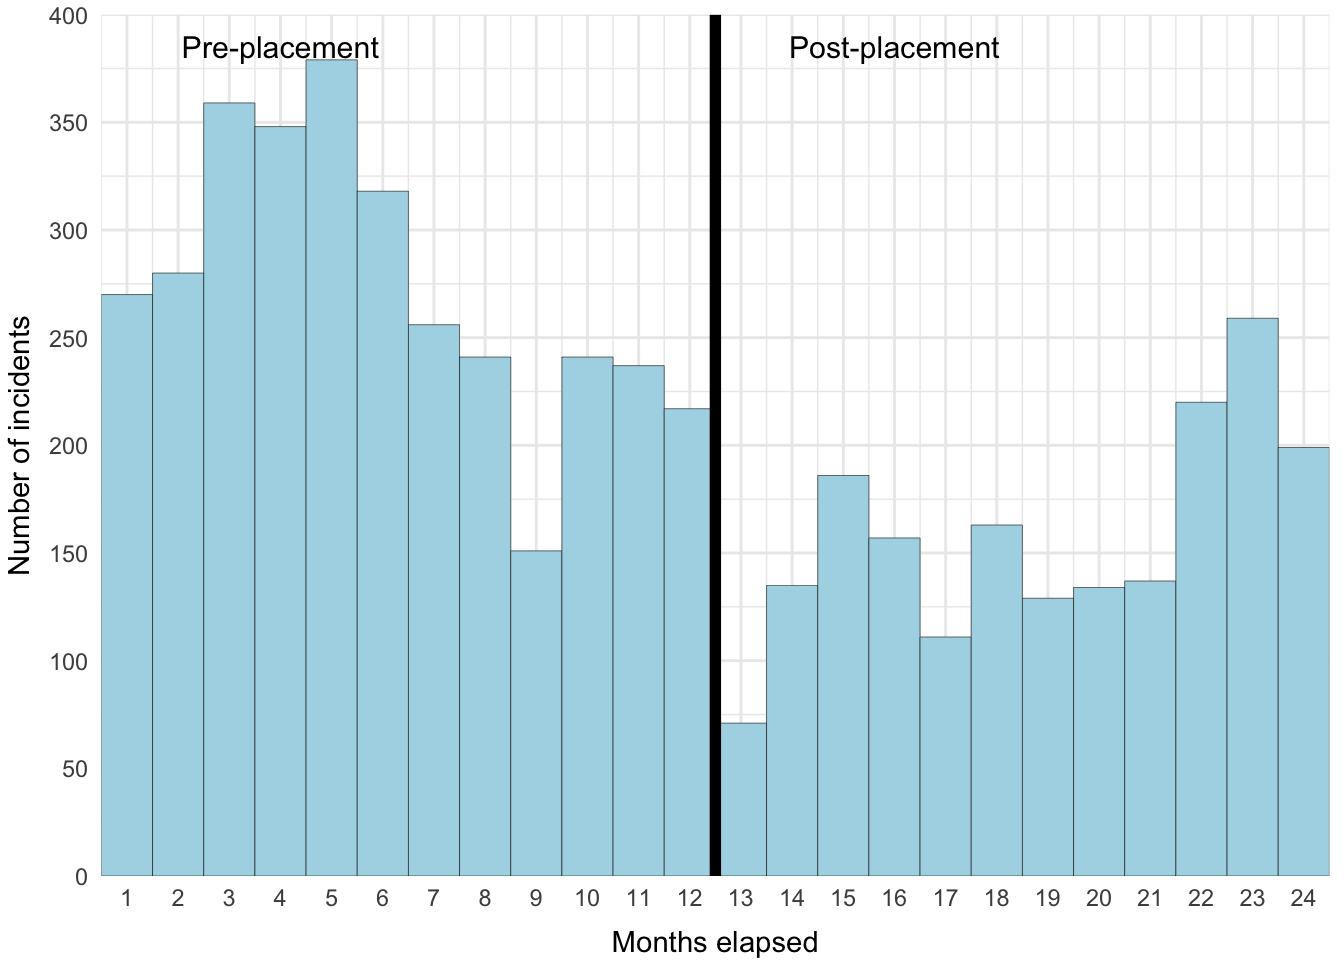
\includegraphics[width=0.9\linewidth]{SPRAINED_files/figure-latex/fig2-1} 

}

\caption{Number of incidents attended by rotation SP in pre- and post-placement phases, stratified by month and SP}\label{fig:fig2}
\end{figure}

Post-rotation, there were also differences in patient call category and acuity based on the NEWS risk category (Figures \ref{fig:fig3} and \ref{fig:fig4}).

\begin{figure}

{\centering 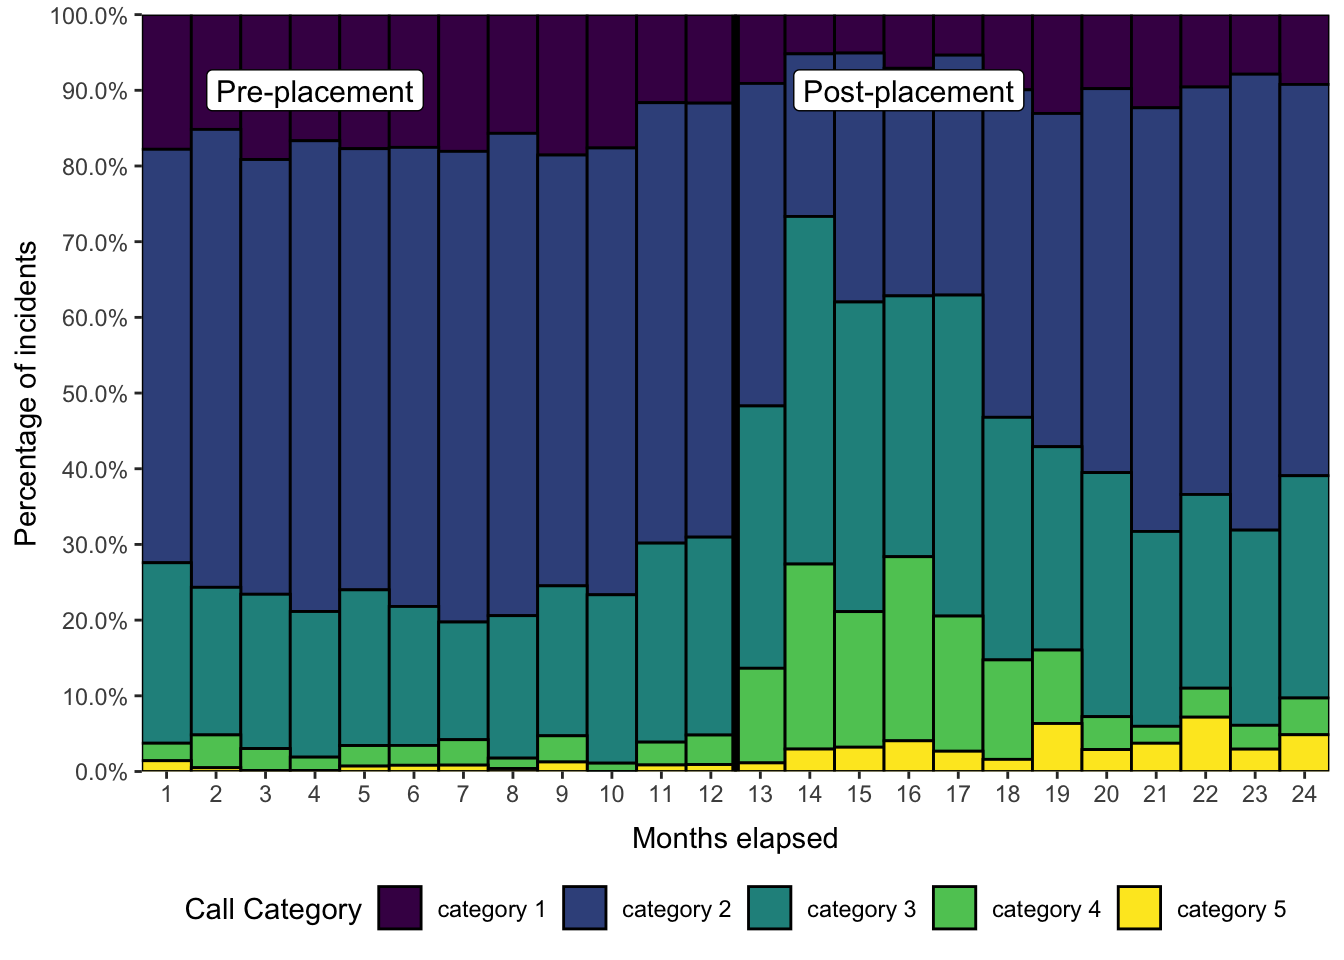
\includegraphics[width=0.9\linewidth]{SPRAINED_files/figure-latex/fig3-1} 

}

\caption{Call category pre- and post-placement}\label{fig:fig3}
\end{figure}

\begin{figure}[p]

{\centering 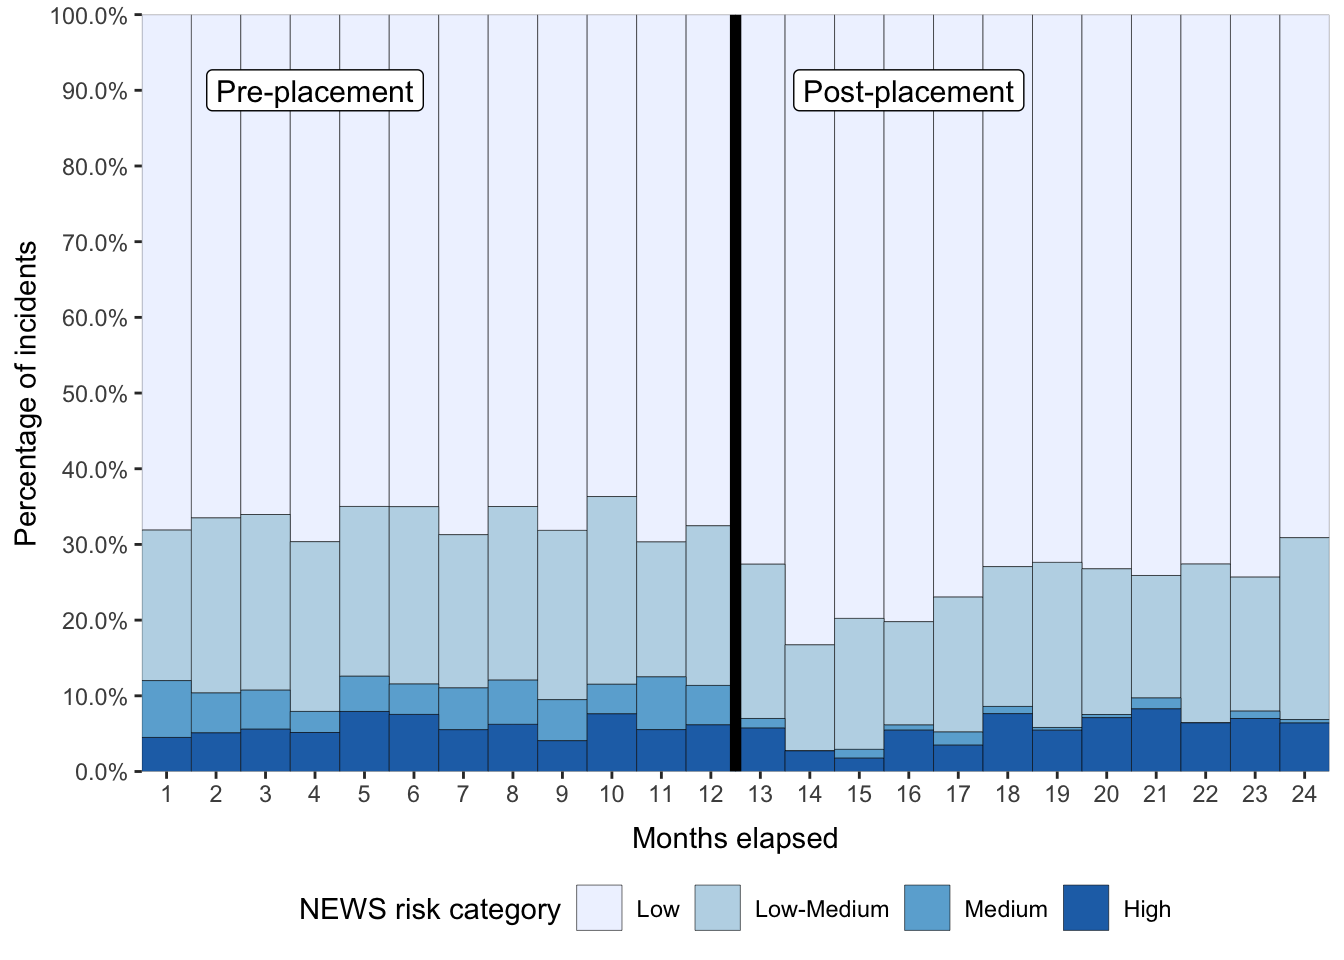
\includegraphics[width=0.9\linewidth]{SPRAINED_files/figure-latex/fig4-1} 

}

\caption{NEWS category pre- and post-placement}\label{fig:fig4}
\end{figure}

\hypertarget{time-series}{%
\subsection*{Time series}\label{time-series}}
\addcontentsline{toc}{subsection}{Time series}

Figure \ref{fig:fig6} illustrates the change in raw and fitted CITS model data between the pre- and post-rotation phase. There was no indication of autoregression (Durbin-Watson statistic 2.37, p=0.79). Post-rotation, the intervention group significantly increased their appropriate non-conveyance rate by 35.0\% (95\%CI 23.8--46.2\%, p=\textless0.001) relative to the control group (Table \ref{tab:cits-table}). However, there was a non-statistically significant decrease in the trend of appropriate non-conveyance relative to the control group of -1.2\% (95\%CI -2.8--0.5\%, p=0.156). Removal of the working impression as a matching variable resulted in a reduction in post-rotation intervention group change in level relative to control group to 27.1\% (95\%CI 16.4--37.7\%, p=\textless0.001), but not trend (-0.9\%, 95\%CI -2.4--0.6\%, p=0.247)

There was an outlier in the intervention group at month 18, but a sensitivity analysis conducted with the data point removed, suggested it had little effect on the post-rotation level and trend of appropriate non-conveyance (36.5\%, 95\%CI 26.3--46.7\%, p=\textless0.001 and -1.2\%, 95\%CI -2.7--0.3\%, p=0.103 respectively).

\begin{figure}

{\centering 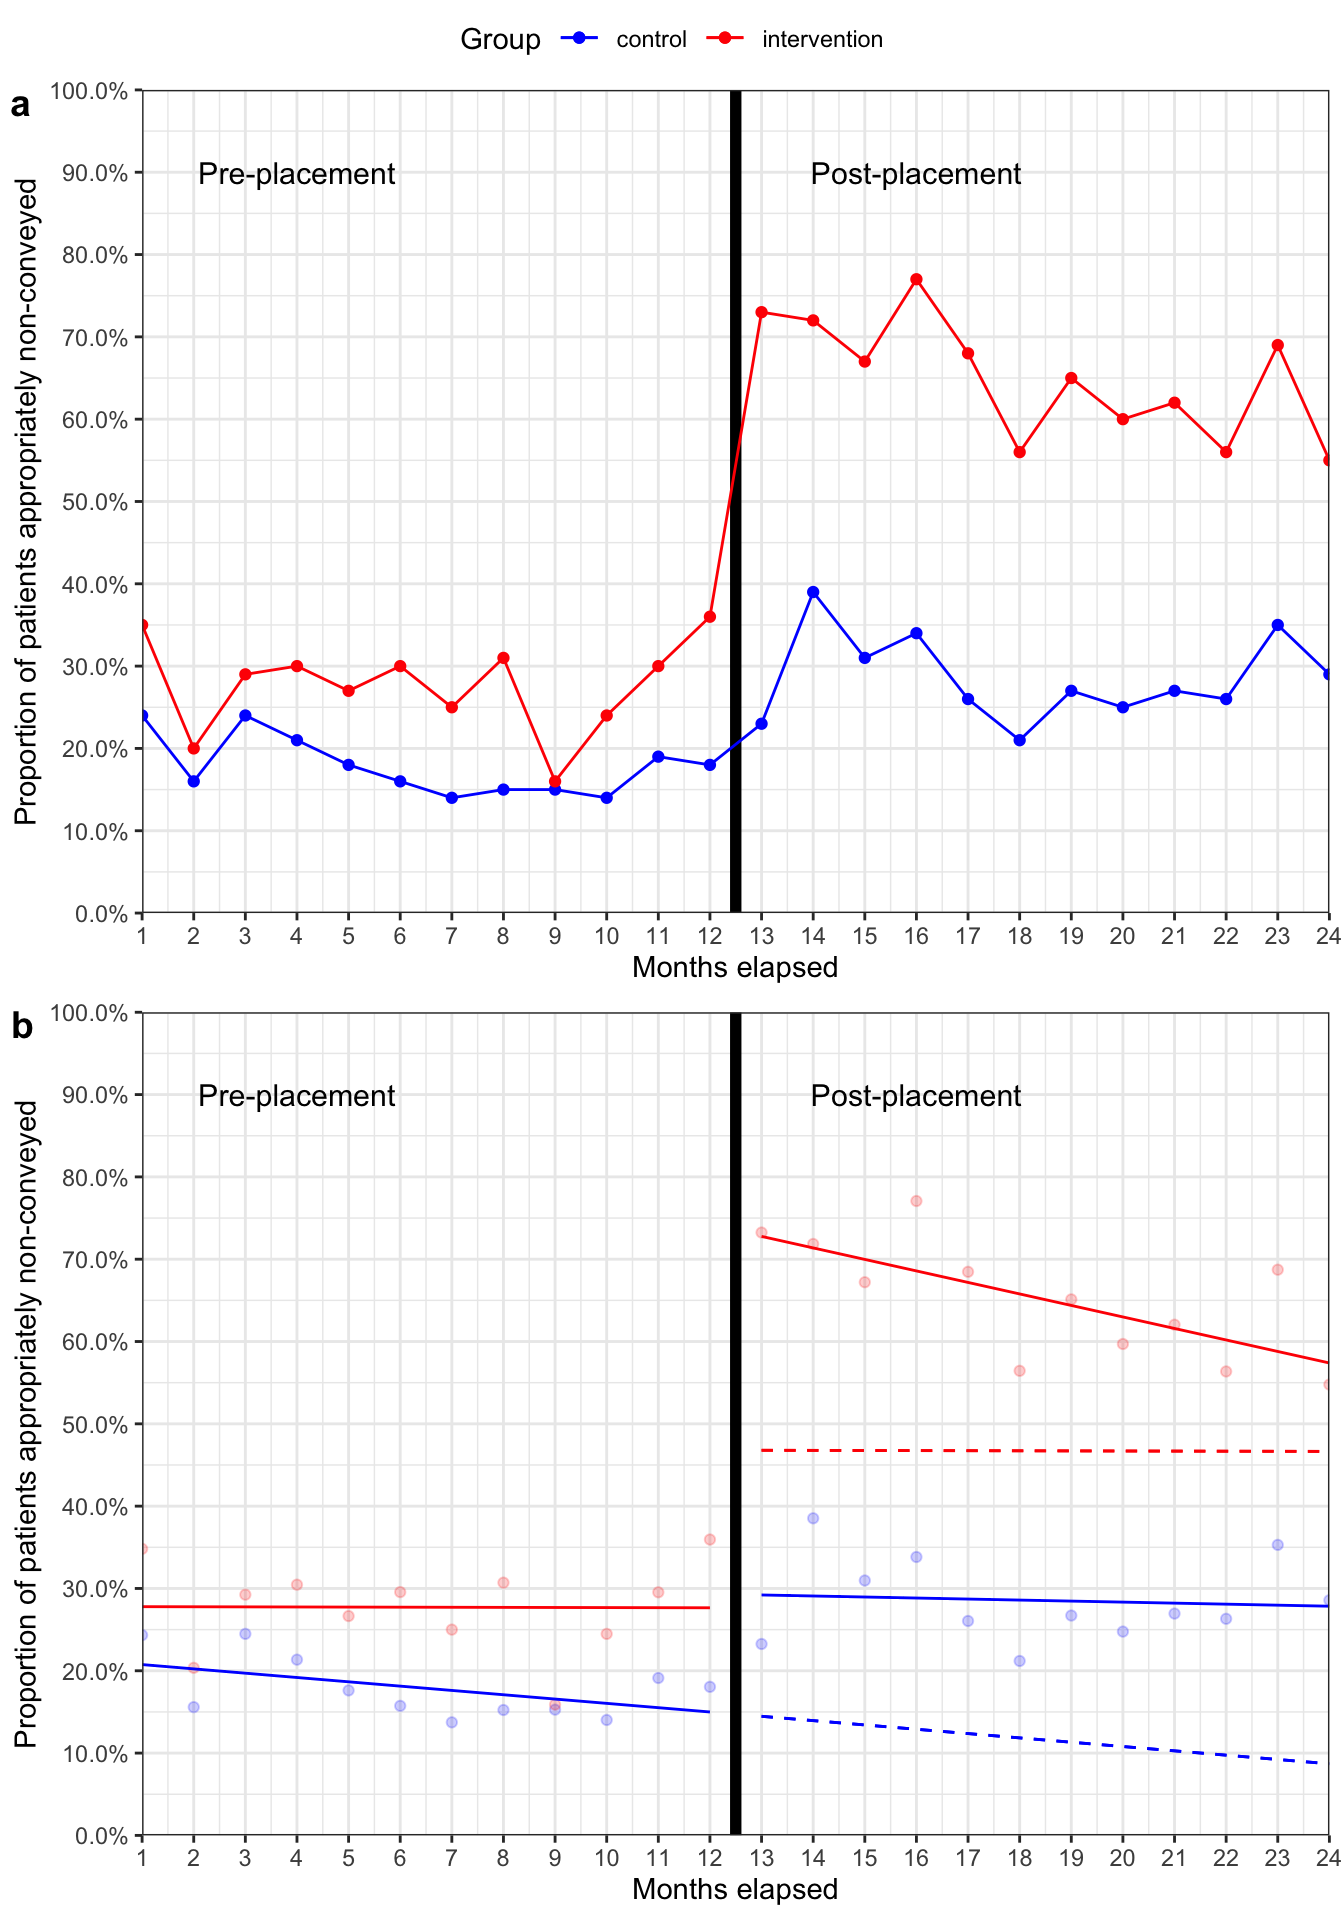
\includegraphics[width=0.9\linewidth]{SPRAINED_files/figure-latex/fig6-1} 

}

\caption{Effect of 10-week primary care rotation on safe non-conveyance. a) Monthly appropriate non-conveyance rates b) Fitted CITS model. Dashed lines represent the counterfactuals.}\label{fig:fig6}
\end{figure}

\begin{longtable}[t]{>{\raggedright\arraybackslash}p{25em}lll}
\caption{\label{tab:cits-table}Result of segmented regression analysis for appropriate non-conveyance}\\
\toprule
  & Coefficient (\%) & 95\% CI & P value\\
\midrule
\endfirsthead
\caption[]{\label{tab:cits-table}Result of segmented regression analysis for appropriate non-conveyance \textit{(continued)}}\\
\toprule
  & Coefficient (\%) & 95\% CI & P value\\
\midrule
\endhead
\
\endfoot
\bottomrule
\endlastfoot
\rowcolor{gray!6}  Initial control group level & 16.8 & 10.9 to 22.8 & <0.001\\
Pre-placement control group trend & 0.1 & -0.7 to 0.9 & 0.831\\
\rowcolor{gray!6}  Difference in level between control and intervention groups & 11.8 & 3.4 to 20.2 & 0.007\\
Intervention group trend relative to control group & -0.3 & -1.4 to 0.9 & 0.622\\
\rowcolor{gray!6}  Post-placement change in control group level & 11.2 & 3.3 to 19.2 & 0.007\\
\addlinespace
Post-placement change in control group trend & 0.1 & -1.0 to 1.2 & 0.862\\
\rowcolor{gray!6}  Post-placement intervention group change in level relative to control group & 35.0 & 23.8 to 46.2 & <0.001\\
Post-placement intervention group change in trend relative to control group & -1.2 & -2.8 to 0.5 & 0.156\\*
\end{longtable}

\hypertarget{economic-analysis}{%
\subsection*{Economic analysis}\label{economic-analysis}}
\addcontentsline{toc}{subsection}{Economic analysis}

Post-rotation, intervention group paramedics cost a mean of £323.71 per incident (95\% CI £318.77--£328.88), compared to £347.79 per incident (95\% CI £343.48--£351.81) for the control group. Cost per appropriate non-conveyance for intervention paramedics was a mean of £509.42 (95\%CI £485.04--£534.97) versus £1124.41 (95\%CI £1042.89--£1216.95) for the control group.

This represents a mean saving of £615 per appropriate non-conveyance (95\%CI £546.43--£687.97) for rotating paramedics compared to the control group.

The sensitivity analysis (excluding working impression) resulted in the post-rotation, intervention group paramedics, costing a mean of £326.31 per incident (95\% CI £321.55--£331.19), versus £345.12 per incident (95\% CI £341.16--£349.14) for the control group. Cost per appropriate non-conveyance for intervention paramedics was a mean of £528.2 (95\%CI £504.11--£554.55) versus £1078.29 (95\%CI £1006.18--£1166.66) for the control group.

\hypertarget{discussion}{%
\section*{Discussion}\label{discussion}}
\addcontentsline{toc}{section}{Discussion}

In this single NHS ambulance service study, we found a clinically and statistical significant increase in appropriate non-conveyance of patients following a 10-week GP rotation. In addition, this intervention proved to be cost saving compared to usual care. These results needs to be interpreted with caution, since they only include data from a single ambulance service with less than 10\% of all paramedics currently in the role of specialist paramedic. Training and experiential opportunities do vary between organisations, in part likely due to the piecemeal way in which the advanced practice roles have evolved for paramedics in the UK {[}\protect\hyperlink{ref-turner_evaluation_2018}{9}{]}. YAS has been commissioning the education of specialist paramedics with local Higher Education Institutions since 2014, with a focus on minor illness and injury, and long-term conditions, which is likely to resonate with other similar schemes {[}\protect\hyperlink{ref-hodge_maintaining_2018}{15}{]}. Furthermore, YAS have continued to work to develop their workforce model aligned to the College of Paramedics post-registration career framework since 2015 {[}\protect\hyperlink{ref-college_of_paramedics_post-registration_2018}{16}{]}.

The non-conveyance rates seen in this study are difficult to compare with other reported statistics, since the population included in this study is different to all emergency call activity. For example, in the pre-placement phase, there was a higher proportion of category 1 and 2 calls (75--76.9\%) compared to figures reported nationally (64\%), but a lower proportion post-placement, due to greater case selection with the introduction of the dedicated SP tasking desk {[}\protect\hyperlink{ref-nhs_england_ambulance_2018}{17}{]}. During the study period, YAS see-and-treat rates were between 22.9--25.4\% which was lower than the English average of 29.3--30.7\% {[}\protect\hyperlink{ref-nhs_england_ambulance_2020}{18}{]}.

An evaluation of the first phase of the rotating paramedic pilot reported non-conveyance rates of at least 70\%, which mirrors the performance of rotating specialist paramedics in Wales {[}\protect\hyperlink{ref-association_of_ambulance_chief_executives_model_2019}{19}{]}. Two sites in the rotating paramedic pilot had non-conveyance rates in excess of 90\%, tended to be primary care focused, rather than fully ambulance service based, highlighting the different interpretation of the guidance issued by Health Education England.

In YAS, the integration into the primary care team for the Leeds rotation, enabled the SPs to develop a greater understanding of the local healthcare system as they navigated pathways across community and acute care. This knowledge was available to be utilised when the SPs rotated back into YAS and were responding to 999 calls in a rapid response car, or working in the EOC to identify appropriate 999 calls for SP response.

\hypertarget{limitations}{%
\subsection*{Limitations}\label{limitations}}
\addcontentsline{toc}{subsection}{Limitations}

It is important to acknowledge this study's limitations. We used routine observational data rather than conducting a randomised-controlled trial for example, which was not possible since the rotation had already completed on commencement of this work. The outcome of this study, while patient focused, could not capture episodes where patients presented to other sectors of the healthcare system as a result of a complication of not being conveyed to hospital. In addition, identifying re-contacts, relied on identification of cases either by NHS number or a combination of patient name, age and incident location which may have been missing on subsequent calls.

The number of missing working impression codes was not anticipated, and so no contingency was made in the methodology to account for this. While the sensitivity analysis showed that this is likely to have had a modest impact on our findings, in retrospect this study would have been more robust with a plan to take account of this.

Finally, it became apparent once the data was provided that determining the grade of paramedic with any certainty was not possible, which may have inflated the performance of the control group by inclusion of specialist paramedics who had not taken part in the GP rotation.

\hypertarget{conclusion-1}{%
\section*{Conclusion}\label{conclusion-1}}
\addcontentsline{toc}{section}{Conclusion}

In this single NHS ambulance service study, we found a clinically and statistical significant increase in appropriate non-conveyance rates by specialist paramedics who had completed a 10-week GP rotation. This improvement persisted for the 12-month period following the rotation and demonstrated cost savings compared to usual care.

\hypertarget{acknowledgements}{%
\subsection*{Acknowledgements}\label{acknowledgements}}
\addcontentsline{toc}{subsection}{Acknowledgements}

This work uses data provided by patients and collected by the NHS as part of their care and support. The authors would also like to thank the Yorkshire Ambulance service business intelligence team who collated the data used in this study.
\emph{Claire Lindsay and Harriet ?}

\hypertarget{contributors}{%
\subsection*{Contributors}\label{contributors}}
\addcontentsline{toc}{subsection}{Contributors}

RP, TY and AH conceived and designed the study. RP obtained the research approvals and acts as guarantor for the paper. All authors drafted the manuscript and contributed substantially to its revision.

\hypertarget{funding}{%
\subsection*{Funding}\label{funding}}
\addcontentsline{toc}{subsection}{Funding}

This paper presents independent research by the NIHR Applied Research Collaboration Yorkshire and Humber (ARC YH).

\hypertarget{disclaimer}{%
\subsection*{Disclaimer}\label{disclaimer}}
\addcontentsline{toc}{subsection}{Disclaimer}

The views expressed in this publication are those of the author(s) and not necessarily those of the National Institute for Health Research or the Department of Health and Social Care.

\hypertarget{appendix-a}{%
\section*{Appendix A}\label{appendix-a}}
\addcontentsline{toc}{section}{Appendix A}

Due to the high number of missing working impressions, we conducted a sensitivity analysis including data that was matched without working impression as a variable. Figure \ref{fig:fig6-no-wi} shows the change in proportion of appropriate non-conveyance in this group and can be compared with \ref{fig:fig6}. The results of the segmented regression can be seen in Table \ref{tab:cits-table-no-wi}.

\begin{figure}

{\centering 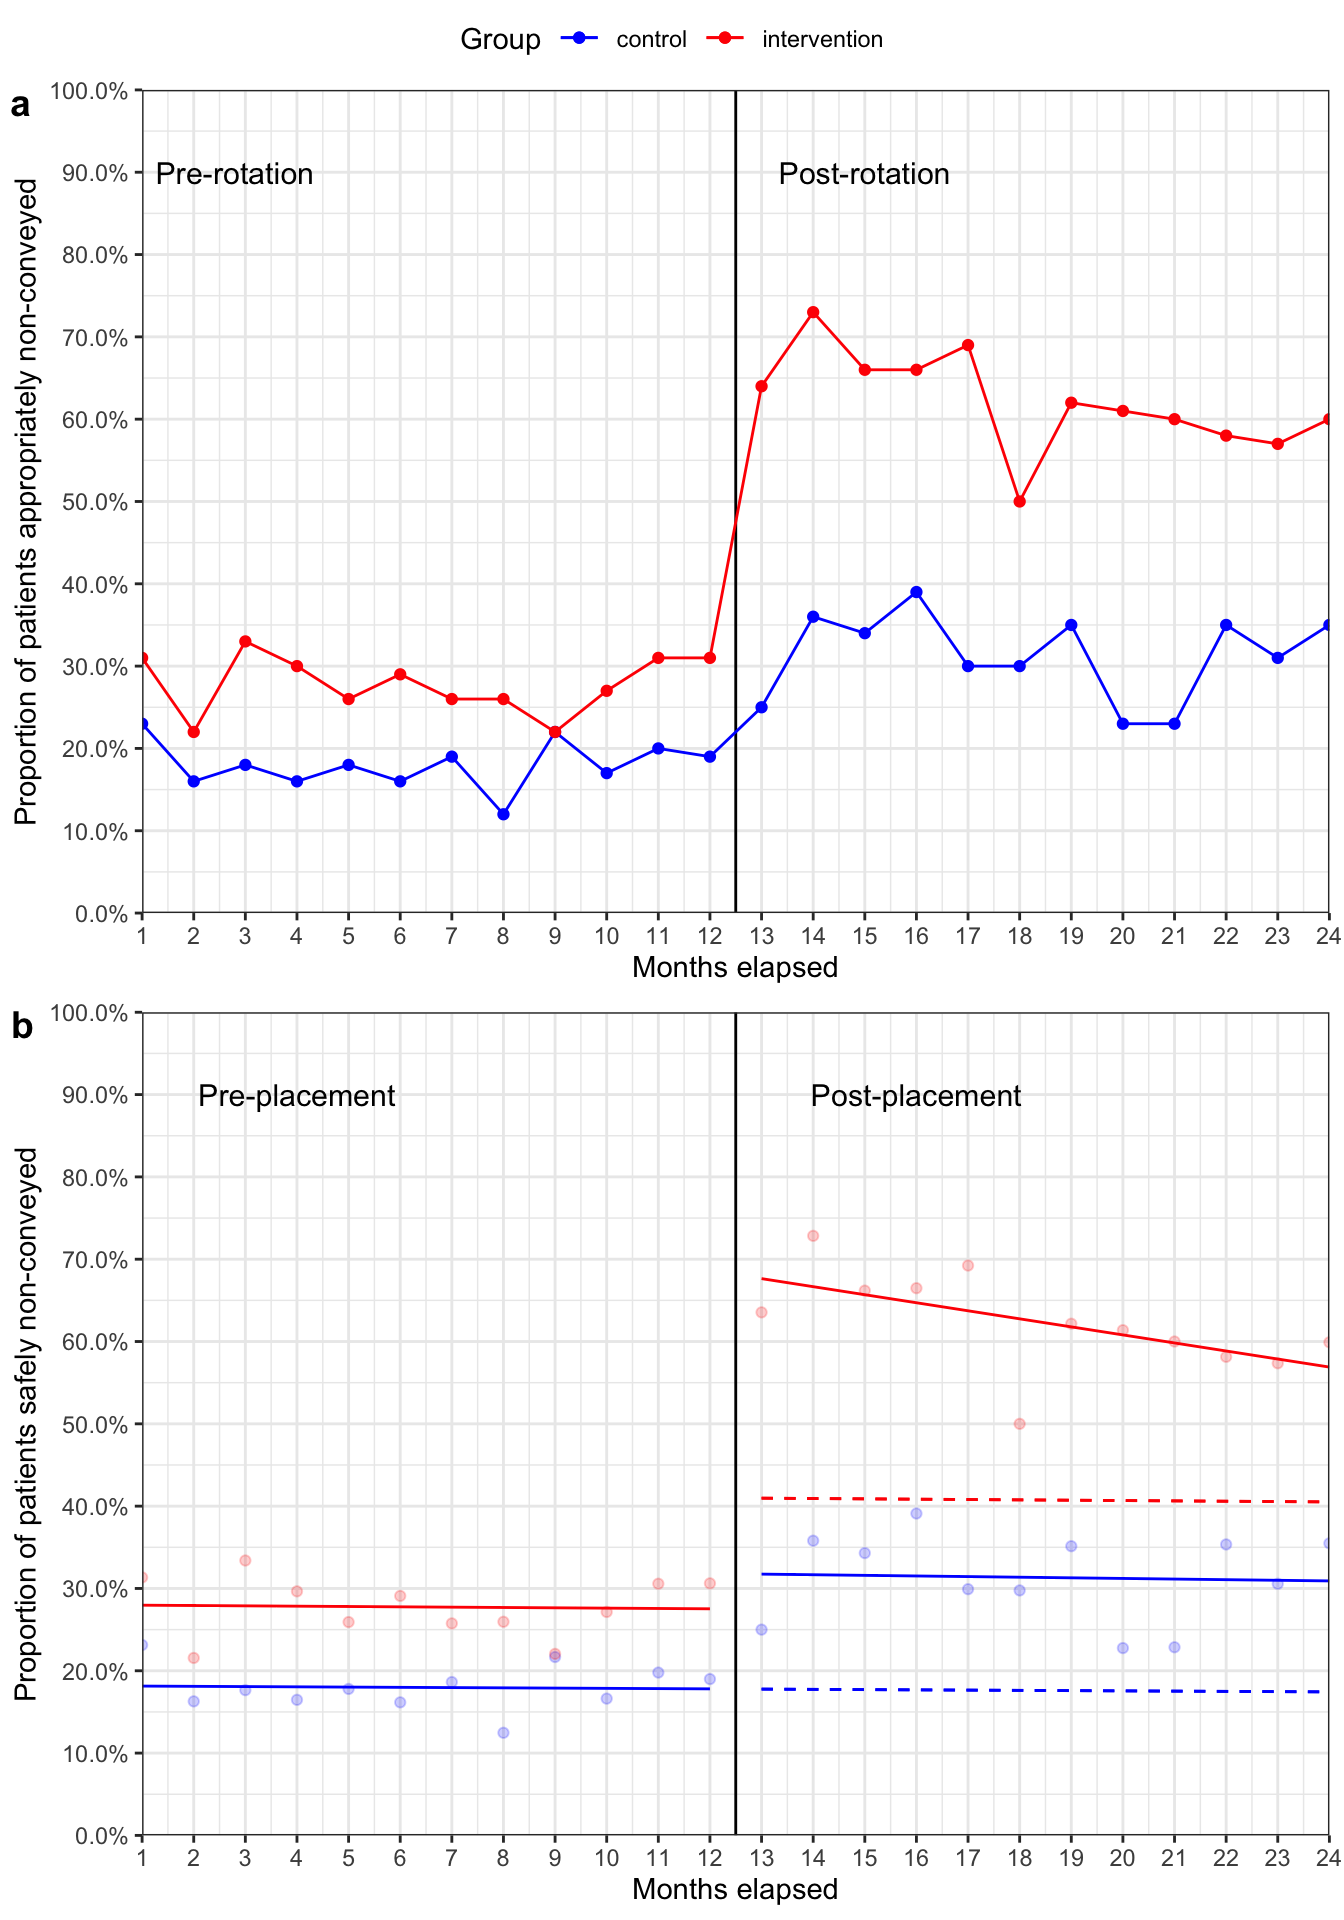
\includegraphics[width=0.9\linewidth]{SPRAINED_files/figure-latex/fig6-no-wi-1} 

}

\caption{Effect of 10-week primary care rotation on safe non-conveyance (excluding working impression). a) Monthly appropriate non-conveyance rates b) Fitted CITS model. Dashed lines represent the counterfactuals.}\label{fig:fig6-no-wi}
\end{figure}

\begin{longtable}[t]{>{\raggedright\arraybackslash}p{25em}lll}
\caption{\label{tab:cits-table-no-wi}Result of segmented regression analysis for appropriate non-conveyance (excluding working impression)}\\
\toprule
  & Coefficient (\%) & 95\% CI & P value\\
\midrule
\endfirsthead
\caption[]{\label{tab:cits-table-no-wi}Result of segmented regression analysis for appropriate non-conveyance (excluding working impression) \textit{(continued)}}\\
\toprule
  & Coefficient (\%) & 95\% CI & P value\\
\midrule
\endhead
\
\endfoot
\bottomrule
\endlastfoot
\rowcolor{gray!6}  Initial control group level & 18.2 & 12.5 to 23.8 & <0.001\\
Pre-rotation control group trend & -0.0 & -0.8 to 0.7 & 0.936\\
\rowcolor{gray!6}  Difference in level between control and intervention groups & 9.9 & 1.9 to 17.8 & 0.017\\
Rotation group trend relative to control group & -0.0 & -1.1 to 1.1 & 0.984\\
\rowcolor{gray!6}  Post-rotation change in control group level & 14.0 & 6.5 to 21.5 & <0.001\\
\addlinespace
Post-rotation change in control group trend & -0.0 & -1.1 to 1.0 & 0.933\\
\rowcolor{gray!6}  Post-rotation intervention group change in level relative to control group & 27.1 & 16.4 to 37.7 & <0.001\\
Post-rotation intervention group change in trend relative to control group & -0.9 & -2.4 to 0.6 & 0.247\\*
\end{longtable}

\hypertarget{references}{%
\section*{References}\label{references}}
\addcontentsline{toc}{section}{References}

\bibliography{SPRAINED-refs.bib}

\hypertarget{refs}{}
\leavevmode\hypertarget{ref-national_audit_office_nhs_2017}{}%
1 National Audit Office. NHS Ambulance Services. National Audit Office. 2017. \url{https://www.nao.org.uk/report/nhs-ambulance-services/} (accessed 22 Oct 2019).

\leavevmode\hypertarget{ref-nhs_england_ambulance_2019}{}%
2 NHS England. Ambulance Quality Indicators Data 2018-19. 2019. \url{https://www.england.nhs.uk/statistics/statistical-work-areas/ambulance-quality-indicators/ambulance-quality-indicators-data-2018-19/} (accessed 22 Oct 2019).

\leavevmode\hypertarget{ref-willett_addressing_2017}{}%
3 Willett K, Benger J. Addressing ambulance handover delays. 2017. \url{https://www.england.nhs.uk/wp-content/uploads/2017/11/ambulance-handover-letter.pdf} (accessed 10 Oct 2019).

\leavevmode\hypertarget{ref-sun_effect_2013}{}%
4 Sun BC, Hsia RY, Weiss RE \emph{et al.} Effect of Emergency Department Crowding on Outcomes of Admitted Patients. \emph{Annals of emergency medicine} 2013;\textbf{61}:605--611.e6. doi:\href{https://doi.org/10.1016/j.annemergmed.2012.10.026}{10.1016/j.annemergmed.2012.10.026}

\leavevmode\hypertarget{ref-guttmann_association_2011}{}%
5 Guttmann A, Schull MJ, Vermeulen MJ \emph{et al.} Association between waiting times and short term mortality and hospital admission after departure from emergency department: Population based cohort study from Ontario, Canada. \emph{BMJ} 2011;\textbf{342}:d2983. doi:\href{https://doi.org/10.1136/bmj.d2983}{10.1136/bmj.d2983}

\leavevmode\hypertarget{ref-bernstein_effect_2009}{}%
6 Bernstein SL, Aronsky D, Duseja R \emph{et al.} The Effect of Emergency Department Crowding on Clinically Oriented Outcomes. \emph{Academic Emergency Medicine} 2009;\textbf{16}:1--10. doi:\href{https://doi.org/10.1111/j.1553-2712.2008.00295.x}{10.1111/j.1553-2712.2008.00295.x}

\leavevmode\hypertarget{ref-richardson_increase_2006}{}%
7 Richardson DB. Increase in patient mortality at 10 days associated with emergency department overcrowding. \emph{The Medical Journal of Australia} 2006;\textbf{184}:213--6.

\leavevmode\hypertarget{ref-mason_developing_2003}{}%
8 Mason S. Developing a community paramedic practitioner intermediate care support scheme for older people with minor conditions. \emph{Emergency Medicine Journal} 2003;\textbf{20}:196--8. doi:\href{https://doi.org/10.1136/emj.20.2.196}{10.1136/emj.20.2.196}

\leavevmode\hypertarget{ref-turner_evaluation_2018}{}%
9 Turner J, Williams J. An Evaluation of early stage development of rotating paramedic model pilot sites. 2018. \url{https://www.hee.nhs.uk/sites/default/files/documents/Feasability\%20Study\%20of\%20the\%20Rotating\%20Paramedics\%20Pilot\%20-\%20Final.pdf} (accessed 10 Oct 2019).

\leavevmode\hypertarget{ref-ocathain_understanding_2018}{}%
10 O'Cathain A, Knowles E, Bishop-Edwards L \emph{et al.} Understanding variation in ambulance service non-conveyance rates: A mixed methods study. \emph{Health Services and Delivery Research} 2018;\textbf{6}:1--192. doi:\href{https://doi.org/10.3310/hsdr06190}{10.3310/hsdr06190}

\leavevmode\hypertarget{ref-sekhon_multivariate_2011}{}%
11 Sekhon JS. Multivariate and Propensity Score Matching Software with Automated Balance Optimization: The Matching package for R. \emph{Journal of Statistical Software} 2011;\textbf{42}:1--52. doi:\href{https://doi.org/10.18637/jss.v042.i07}{10.18637/jss.v042.i07}

\leavevmode\hypertarget{ref-mitchell_introduction_1996}{}%
12 Mitchell M. \emph{An introduction to genetic algorithms}. Cambridge, Mass:: MIT Press 1996.

\leavevmode\hypertarget{ref-penfold_use_2013}{}%
13 Penfold RB, Zhang F. Use of Interrupted Time Series Analysis in Evaluating Health Care Quality Improvements. \emph{Academic Pediatrics} 2013;\textbf{13}:S38--44. doi:\href{https://doi.org/10.1016/j.acap.2013.08.002}{10.1016/j.acap.2013.08.002}

\leavevmode\hypertarget{ref-nhs_improvement_reference_2018}{}%
14 NHS Improvement. Reference Costs. 2018. \url{https://improvement.nhs.uk/resources/reference-costs/} (accessed 28 Nov 2019).

\leavevmode\hypertarget{ref-hodge_maintaining_2018}{}%
15 Hodge A, Swift S, Wilson JP. Maintaining competency: A qualitative study of clinical supervision and mentorship as a framework for specialist paramedics. \emph{British Paramedic Journal} 2018;\textbf{3}:10--5. doi:\href{https://doi.org/10.29045/14784726.2018.12.3.3.10}{10.29045/14784726.2018.12.3.3.10}

\leavevmode\hypertarget{ref-college_of_paramedics_post-registration_2018}{}%
16 College of Paramedics. Post-registration paramedic career framework - 4th edition. 2018. \url{https://collegeofparamedics.co.uk/COP/ProfessionalDevelopment/post_reg_career_framework.aspx} (accessed 1 Jun 2020).

\leavevmode\hypertarget{ref-nhs_england_ambulance_2018}{}%
17 NHS England. Ambulance Response Programme Review. 2018. \url{https://www.england.nhs.uk/wp-content/uploads/2018/10/ambulance-response-programme-review.pdf} (accessed 1 Jun 2020).

\leavevmode\hypertarget{ref-nhs_england_ambulance_2020}{}%
18 NHS England. Ambulance Quality Indicators. 2020. \url{https://www.england.nhs.uk/statistics/statistical-work-areas/ambulance-quality-indicators/} (accessed 1 Jun 2020).

\leavevmode\hypertarget{ref-association_of_ambulance_chief_executives_model_2019}{}%
19 Association of Ambulance Chief Executives. Model of rotational working aims to stop ambulance trusts spinning out of control - aace.org.uk. 2019. \url{https://aace.org.uk/news/model-of-rotational-working-aims-to-stop-ambulance-trusts-spinning-out-of-control/} (accessed 1 Jun 2020).

\end{document}
